% Standalone version - CORRECTED
% pdflatex temporal_registration_flowchart_standalone.tex

\documentclass[border=10pt]{standalone}
\usepackage{tikz}
\usetikzlibrary{shapes.geometric, arrows.meta, positioning, calc}

\begin{document}
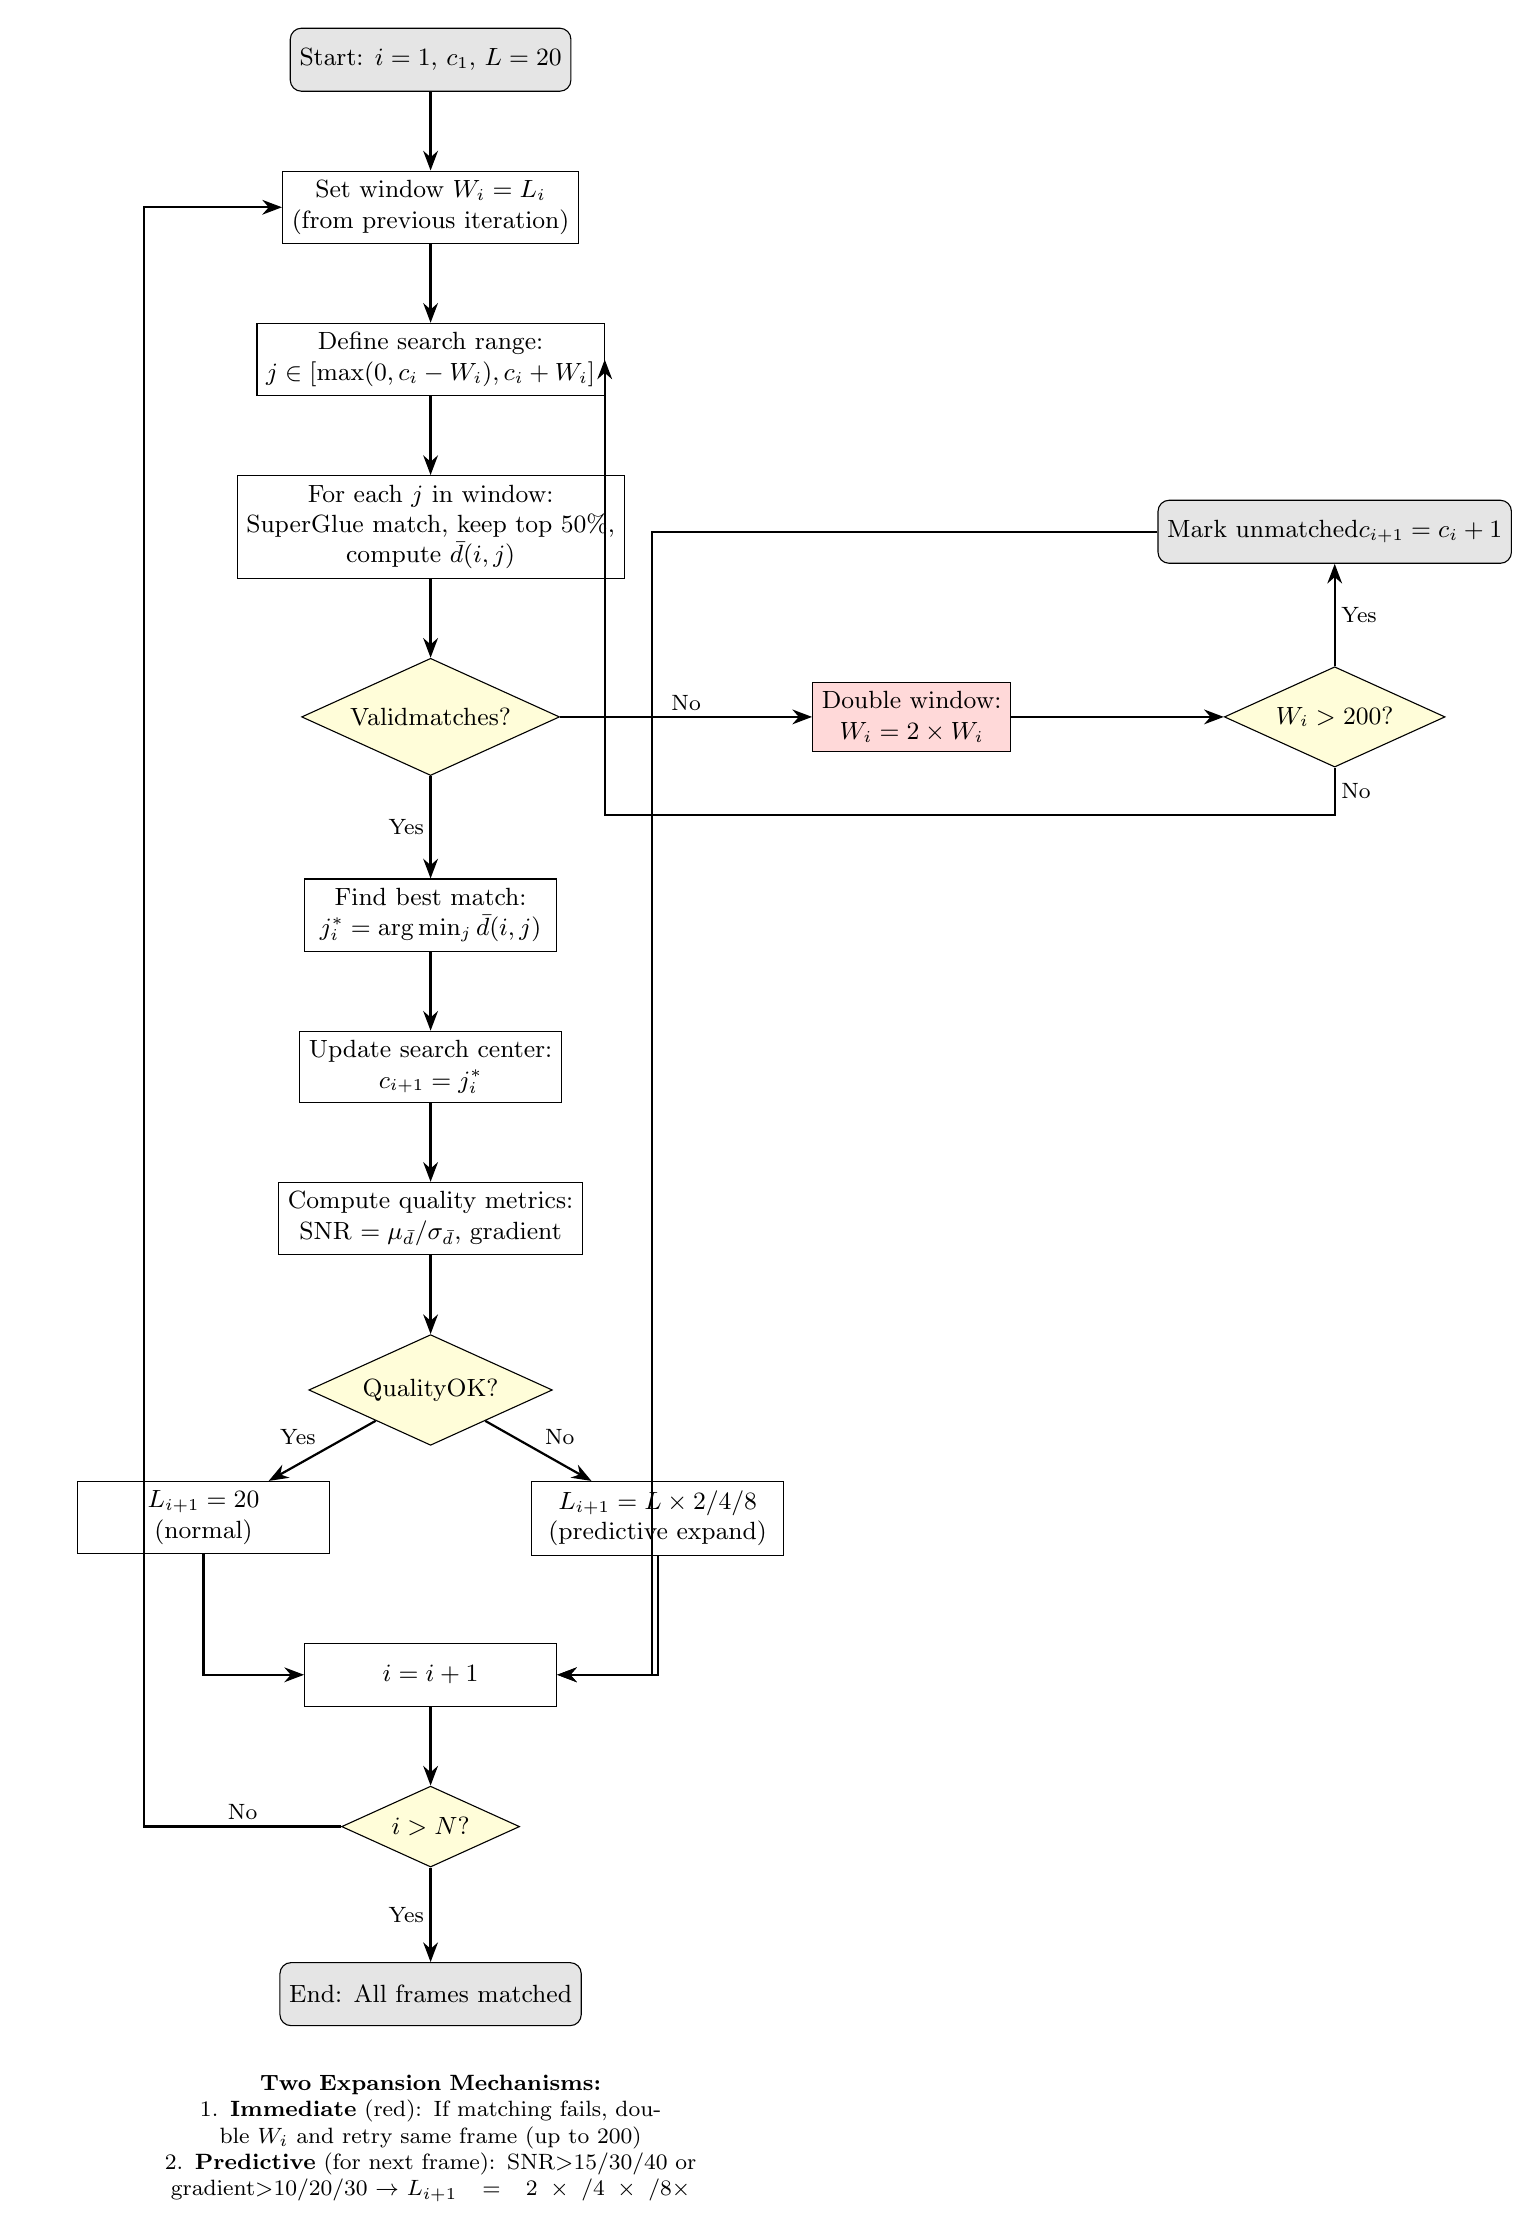
\begin{tikzpicture}[
    node distance=1.0cm and 2.2cm,
    startstop/.style={rectangle, rounded corners, minimum width=3cm, minimum height=0.8cm, text centered, draw=black, fill=gray!20, font=\small},
    process/.style={rectangle, minimum width=3.2cm, minimum height=0.8cm, text centered, draw=black, fill=white, font=\small, align=center},
    decision/.style={diamond, aspect=2.2, minimum width=2cm, text centered, draw=black, fill=yellow!15, font=\small},
    expand/.style={rectangle, minimum width=2.5cm, minimum height=0.8cm, text centered, draw=black, fill=red!15, font=\small, align=center},
    arrow/.style={-{Stealth[length=2.5mm]}, thick},
    label/.style={font=\footnotesize, fill=white, inner sep=2pt}
]

% === START ===
\node (start) [startstop] {Start: $i=1$, $c_1$, $L=20$};

% === MAIN LOOP ===
\node (setwindow) [process, below=of start] {Set window $W_i = L_i$\\(from previous iteration)};

\node (search) [process, below=of setwindow] {Define search range:\\$j \in [\max(0, c_i - W_i), c_i + W_i]$};

\node (matchloop) [process, below=of search] {For each $j$ in window:\\SuperGlue match, keep top 50\%,\\compute $\bar{d}(i,j)$};

\node (checkmatch) [decision, below=of matchloop] {Valid\\matches?};

% === IMMEDIATE EXPANSION (right branch) ===
\node (expand1) [expand, right=of checkmatch, xshift=1.0cm] {Double window:\\$W_i = 2 \times W_i$};
\node (checkmax) [decision, right=of expand1, xshift=0.5cm] {$W_i > 200$?};
\node (fail) [startstop, above=of checkmax, yshift=0.3cm] {Mark unmatched\\$c_{i+1} = c_i + 1$};

% === SUCCESS PATH ===
\node (findmin) [process, below=of checkmatch, yshift=-0.3cm] {Find best match:\\$j^*_i = \arg\min_j \bar{d}(i,j)$};

\node (update) [process, below=of findmin] {Update search center:\\$c_{i+1} = j^*_i$};

\node (metrics) [process, below=of update] {Compute quality metrics:\\SNR $= \mu_{\bar{d}} / \sigma_{\bar{d}}$, gradient};

\node (predictive) [decision, below=of metrics] {Quality\\OK?};

\node (setnormal) [process, below left=0.8cm and 0.5cm of predictive] {$L_{i+1} = 20$\\(normal)};
\node (setexpand) [process, below right=0.8cm and 0.5cm of predictive] {$L_{i+1} = L \times 2/4/8$\\(predictive expand)};

\node (increment) [process, below=2.5cm of predictive] {$i = i + 1$};

\node (checkend) [decision, below=of increment] {$i > N$?};

\node (stop) [startstop, below=of checkend, yshift=-0.2cm] {End: All frames matched};

% === ARROWS - Main flow ===
\draw [arrow] (start) -- (setwindow);
\draw [arrow] (setwindow) -- (search);
\draw [arrow] (search) -- (matchloop);
\draw [arrow] (matchloop) -- (checkmatch);

% No match -> immediate expansion
\draw [arrow] (checkmatch) -- node[label, above] {No} (expand1);
\draw [arrow] (expand1) -- (checkmax);
\draw [arrow] (checkmax) -- node[label, right] {Yes} (fail);
\draw [arrow] (checkmax.south) -- node[label, right] {No} ++(0,-0.6) -| (search.east);
\draw [arrow] (fail) -| ($(increment.east)+(1.2,0)$) -- (increment.east);

% Match found -> success path
\draw [arrow] (checkmatch) -- node[label, left] {Yes} (findmin);
\draw [arrow] (findmin) -- (update);
\draw [arrow] (update) -- (metrics);
\draw [arrow] (metrics) -- (predictive);

% Predictive window sizing
\draw [arrow] (predictive) -- node[label, above left] {Yes} (setnormal);
\draw [arrow] (predictive) -- node[label, above right] {No} (setexpand);
\draw [arrow] (setnormal) |- (increment);
\draw [arrow] (setexpand) |- (increment);

\draw [arrow] (increment) -- (checkend);
\draw [arrow] (checkend) -- node[label, left] {Yes} (stop);

% Loop back
\draw [arrow] (checkend.west) -- node[label, above] {No} ++(-2.5,0) |- (setwindow.west);

% === LEGEND ===
\node [below=0.5cm of stop, font=\footnotesize, text width=10cm, align=center] {
    \textbf{Two Expansion Mechanisms:}\\
    1. \textbf{Immediate} (red): If matching fails, double $W_i$ and retry same frame (up to 200)\\
    2. \textbf{Predictive} (for next frame): SNR$>$15/30/40 or gradient$>$10/20/30 $\rightarrow$ $L_{i+1} = 2\times/4\times/8\times$
};

\end{tikzpicture}
\end{document}
